\section{Initial interviews}\label{sec:initialInterviews}
	\subsection{Teacher Interview}
		\begin{itemize}
		\item[-] Educational level of the teacher 
		\item[-] Describe a typical class + homework
		\item[-] Which areas withing music is taught (theory, instruments, genres etc.)
		\item[-] Tools and materials(Digital as well as analog, iPads, apps, books, instruments, syntesizers and the incorporation in the class)
		\item[-] Methods used (Didaktiske model)
		\item[-] Shortcommings and keeping the engagement of the children
		\item[-] Gamification in the classroom
		\item[-] Difference in lectures from grade to grade
		\item[-] Which role the teacher plays, if they're active role or more passive
		\end{itemize}
	
\section{A List of design suggestions- outcome of the Crawford slip method}\label{CrawfordSlipList}
Things to have in mind when designing our tool
[ this is a list of brainstormed topics and areas, for which we believe (based on the analysis, including the workshop at Sankt Annæ) should be discussed during the design process. The list is setup as suggestions for the design, and as so, not every aspect is required to go onto the design!]

Collaboration:
\begin{itemize}
\item	The students should work together in achieving the goal. (Each student is part of a bigger picture.)
\item	The tool could be used on a dynamic number of students to achieve variation. 
\item	The students could be collaborating by helping each other. 
\item	The students could teach each other, as this is a good way of gaining a better understanding for both students. 
\item	The use of the tool could be turn based.
\item	Turn based collaboration could be used for complexity management.
\item	The tool could control the turn taking. 
\item	A chosen leader of the group could encourage collaboration.
\item	A leader role would fit with the idea of Belbin’s team roles, which relates to group dynamics. 
\item	If each student has a specific role, no one can control the tool alone. Everyone must collaborate. 
\item	A chosen leader role could be turn based.
\item	The task(s) for one student could overlap with the next students task(s), enhancing collaboration. 
\item	The students could be collaborating by “battling” each other (Constructive competition).
\item	Be careful that competition does not result in an unconstructive competitive collaboration. 
\item	Competition and gamification can be used together. 
\item	 Gamification can be used. 
\end{itemize}

Tool specifications and functionalities:
\begin{itemize}
\item	The tool could concern music- creation, - performance, or/and – understanding.
\item	If specific instruments are used in the tool (“playing” piano), the instruments playability could be visualized. E.g. for drums the interface could be round touchpads arranged and sized inspired by a real drum set. 
\item	Pitch could be visualized by moving up/down or away/closer. 
\item	Colors used for the tool should be chosen carefully. 
\item	Pure toes could be used to learn basic and more complex understandings, (rhythm, pitch .. ) 
\item	Pure tones might be best to gain an understanding of the connection between pitch. (it might be more difficult to learn the same with complex tones)
\item	Complex sounds could be used to learn rhythm. 
\item	A limited possibility to change sound, rhythm or alike, could make the tool boring. 
\item	Too many repetitions might become boring. 
\item	The tool could make it possible to “play” an instrument without actually playing the instrument (simulation/ using the sounds of the instrument). 
\item	Using game elements might enhance motivation.
\item	The tool could use the “hear and repeat” approach. 
\item	The tool might want to have a clear purpose in order to relate to the education. 
\item	The tool could make the students able to control and shape sound (rhythm, pitch, and more).
\item	The tool could be a sequencer for the students to manipulate sounds. 
\item	The tool could be task based. 
\item	The tool could enhance creativity by facilitate Fri Leg
\item	Fri leg could enhance variation. 
\item	By making the tool somehow wearable, the felling of involvement might be enhanced. Being part of the music.
\item	The tool could strive to make the students involved/part of the music instead of listeners.
\item	The tool size might have to be considered in relation to classroom setting. 
\item	For getting as must time of usage the time for setting up/ getting ready is ideal if low. 
\item	If the size is relatively small the classroom arrangement does not need to be changed – setup time reduced. 
\item	A larger tool could mean that there is room for movement– movement has been facilitated. 
\item	A large tool might not fit in a classroom environment.
\item	The tool could strive to be considered comfy to use.   
\item	The tools interface could strive to be intuitive and simple.
\item	Movement could be used to control or alter the sound. 
\item	Movement could be used to understand elements of music. (learning by doing) 
\end{itemize}


\begin{figure}[H]
	\centering
	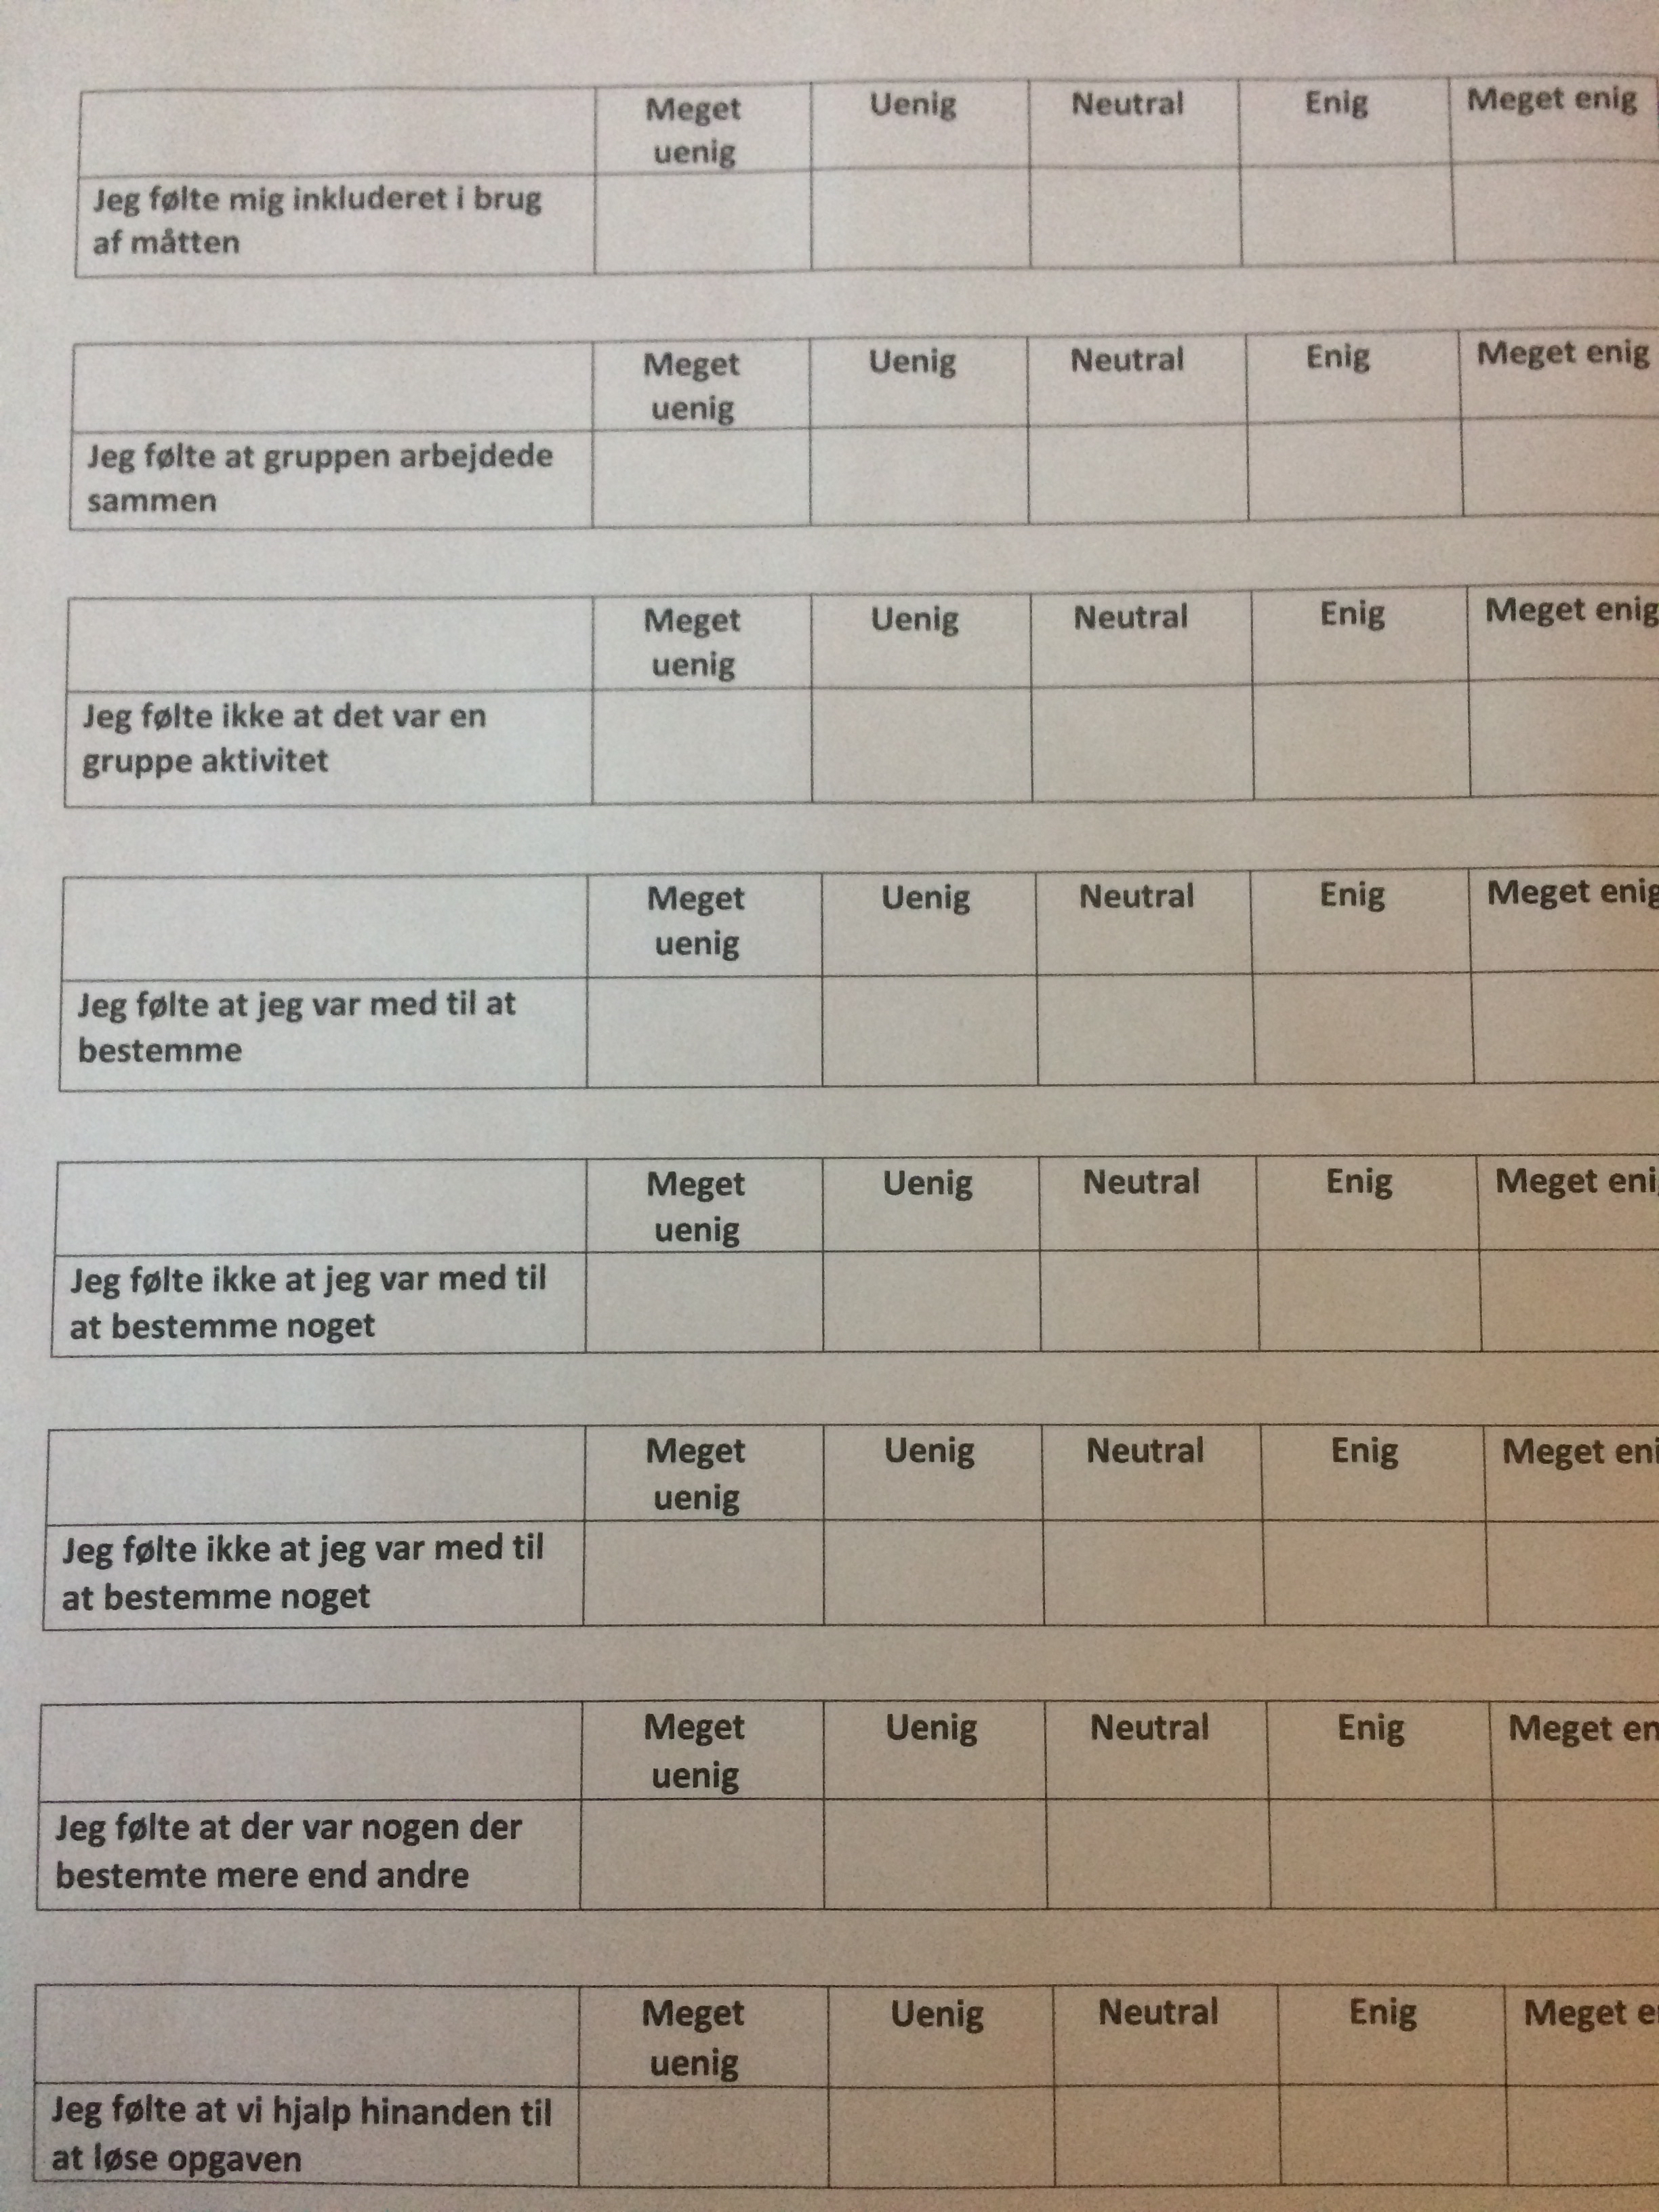
\includegraphics[width=0.7\linewidth]{figure/Appendices/likerts}
	\caption{Likert scale from Skt. Annæ}
	\label{fig:likertScale}
\end{figure}

\section{Test papers}\label{sec:testPaper})
    \begin{figure}[H]
		\centering
		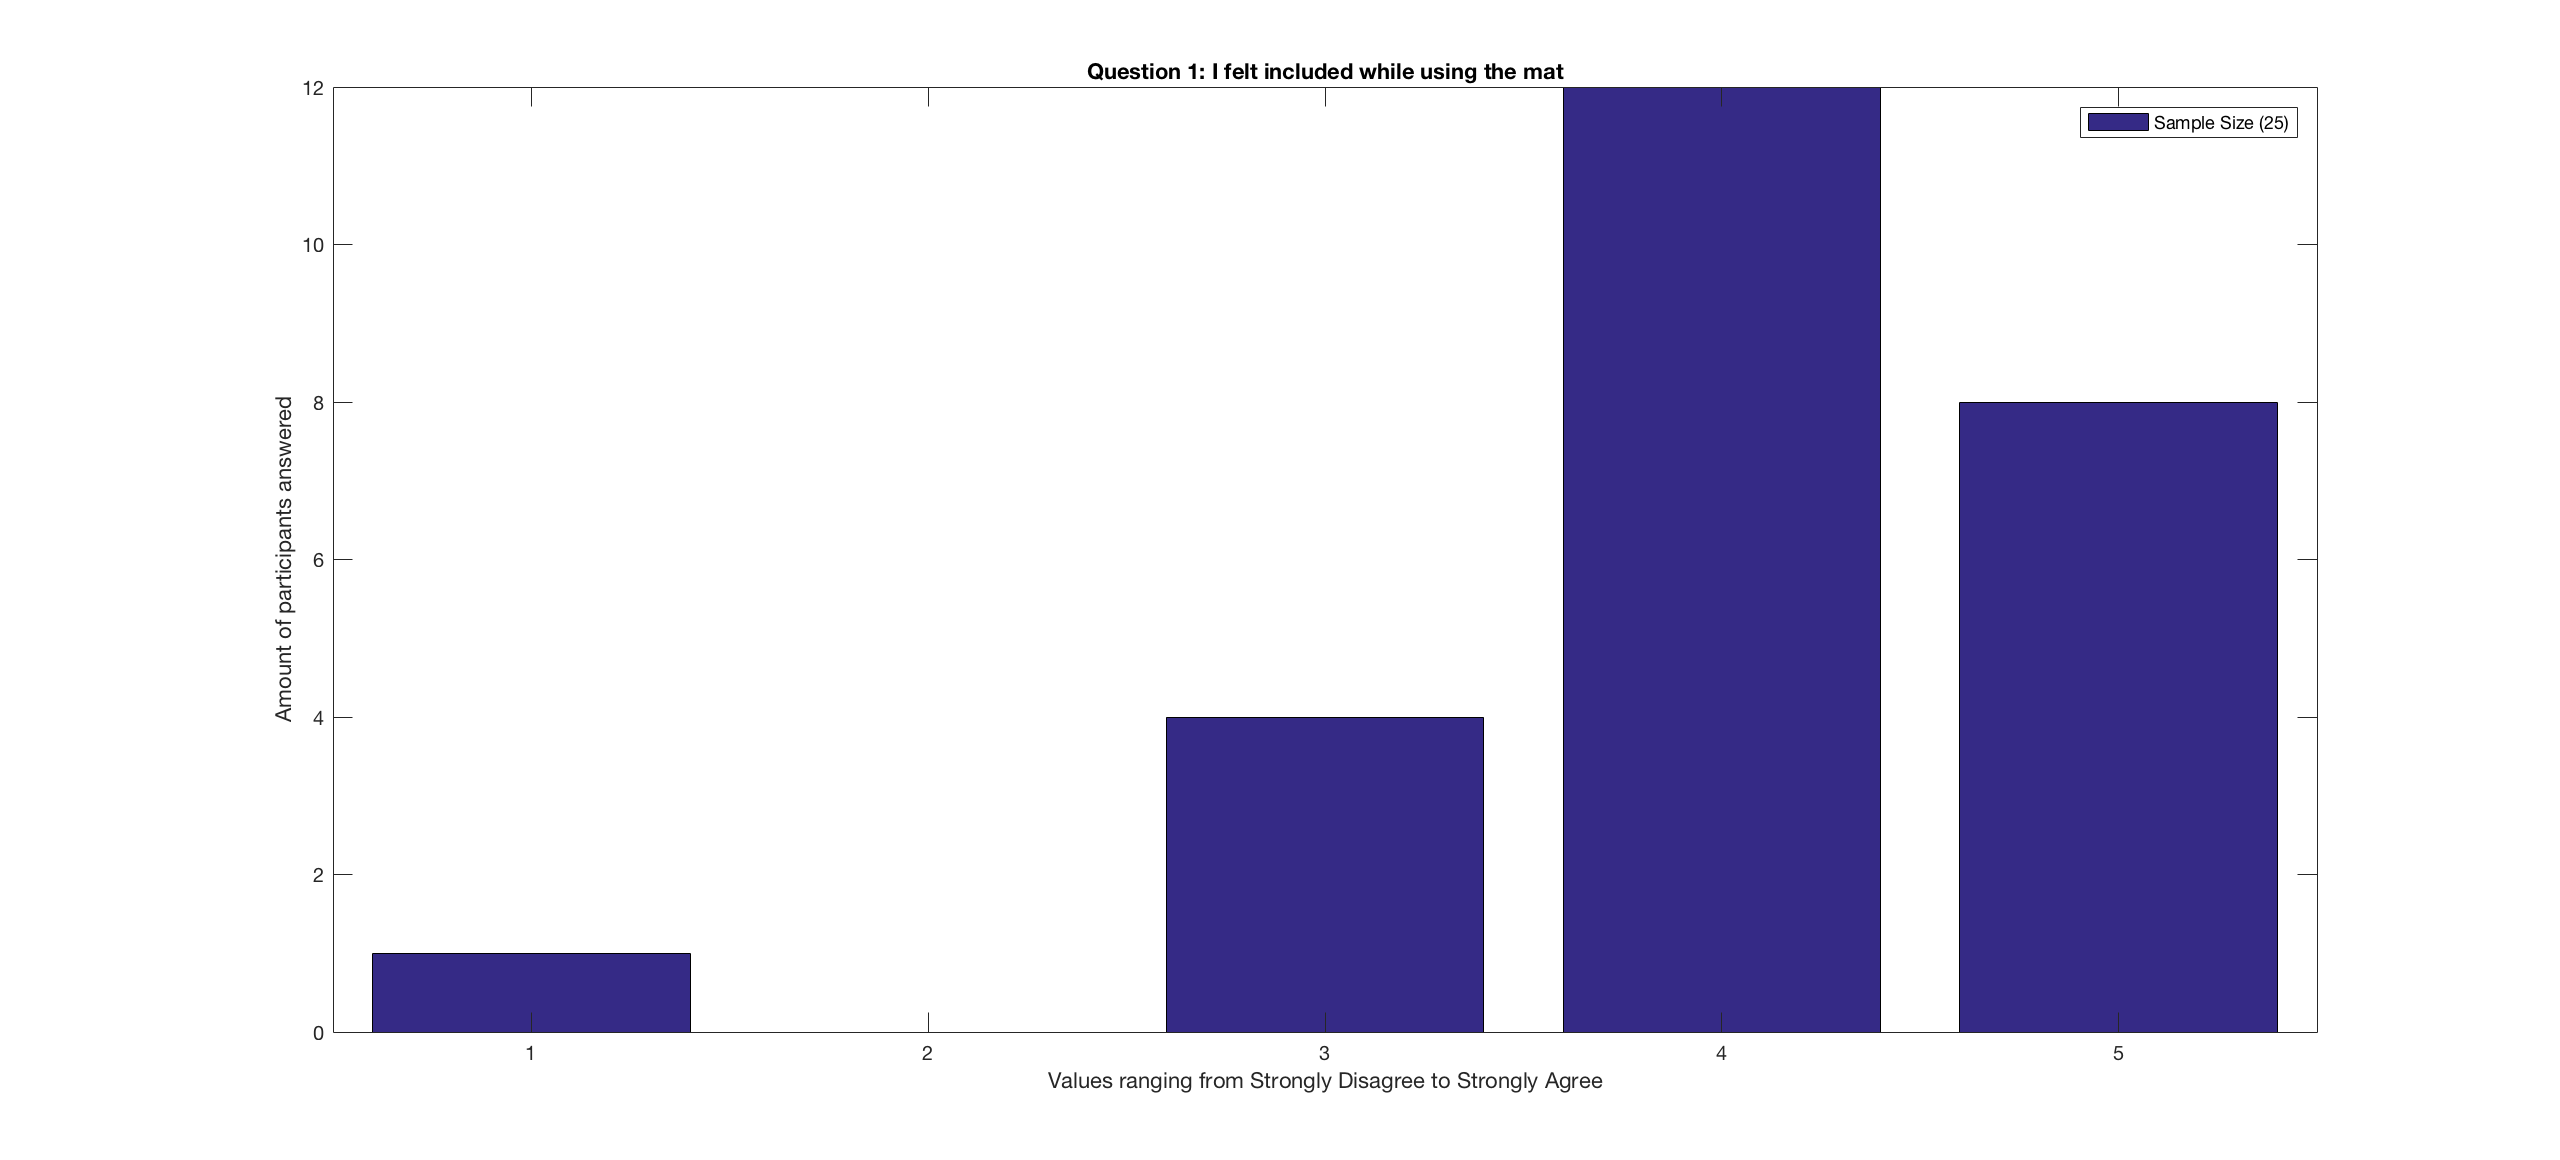
\includegraphics[width=0.9\linewidth]{figure/Appendices/Question1} 
		\caption{Question1}
	\end{figure}

    \begin{figure}[H]
		\centering
		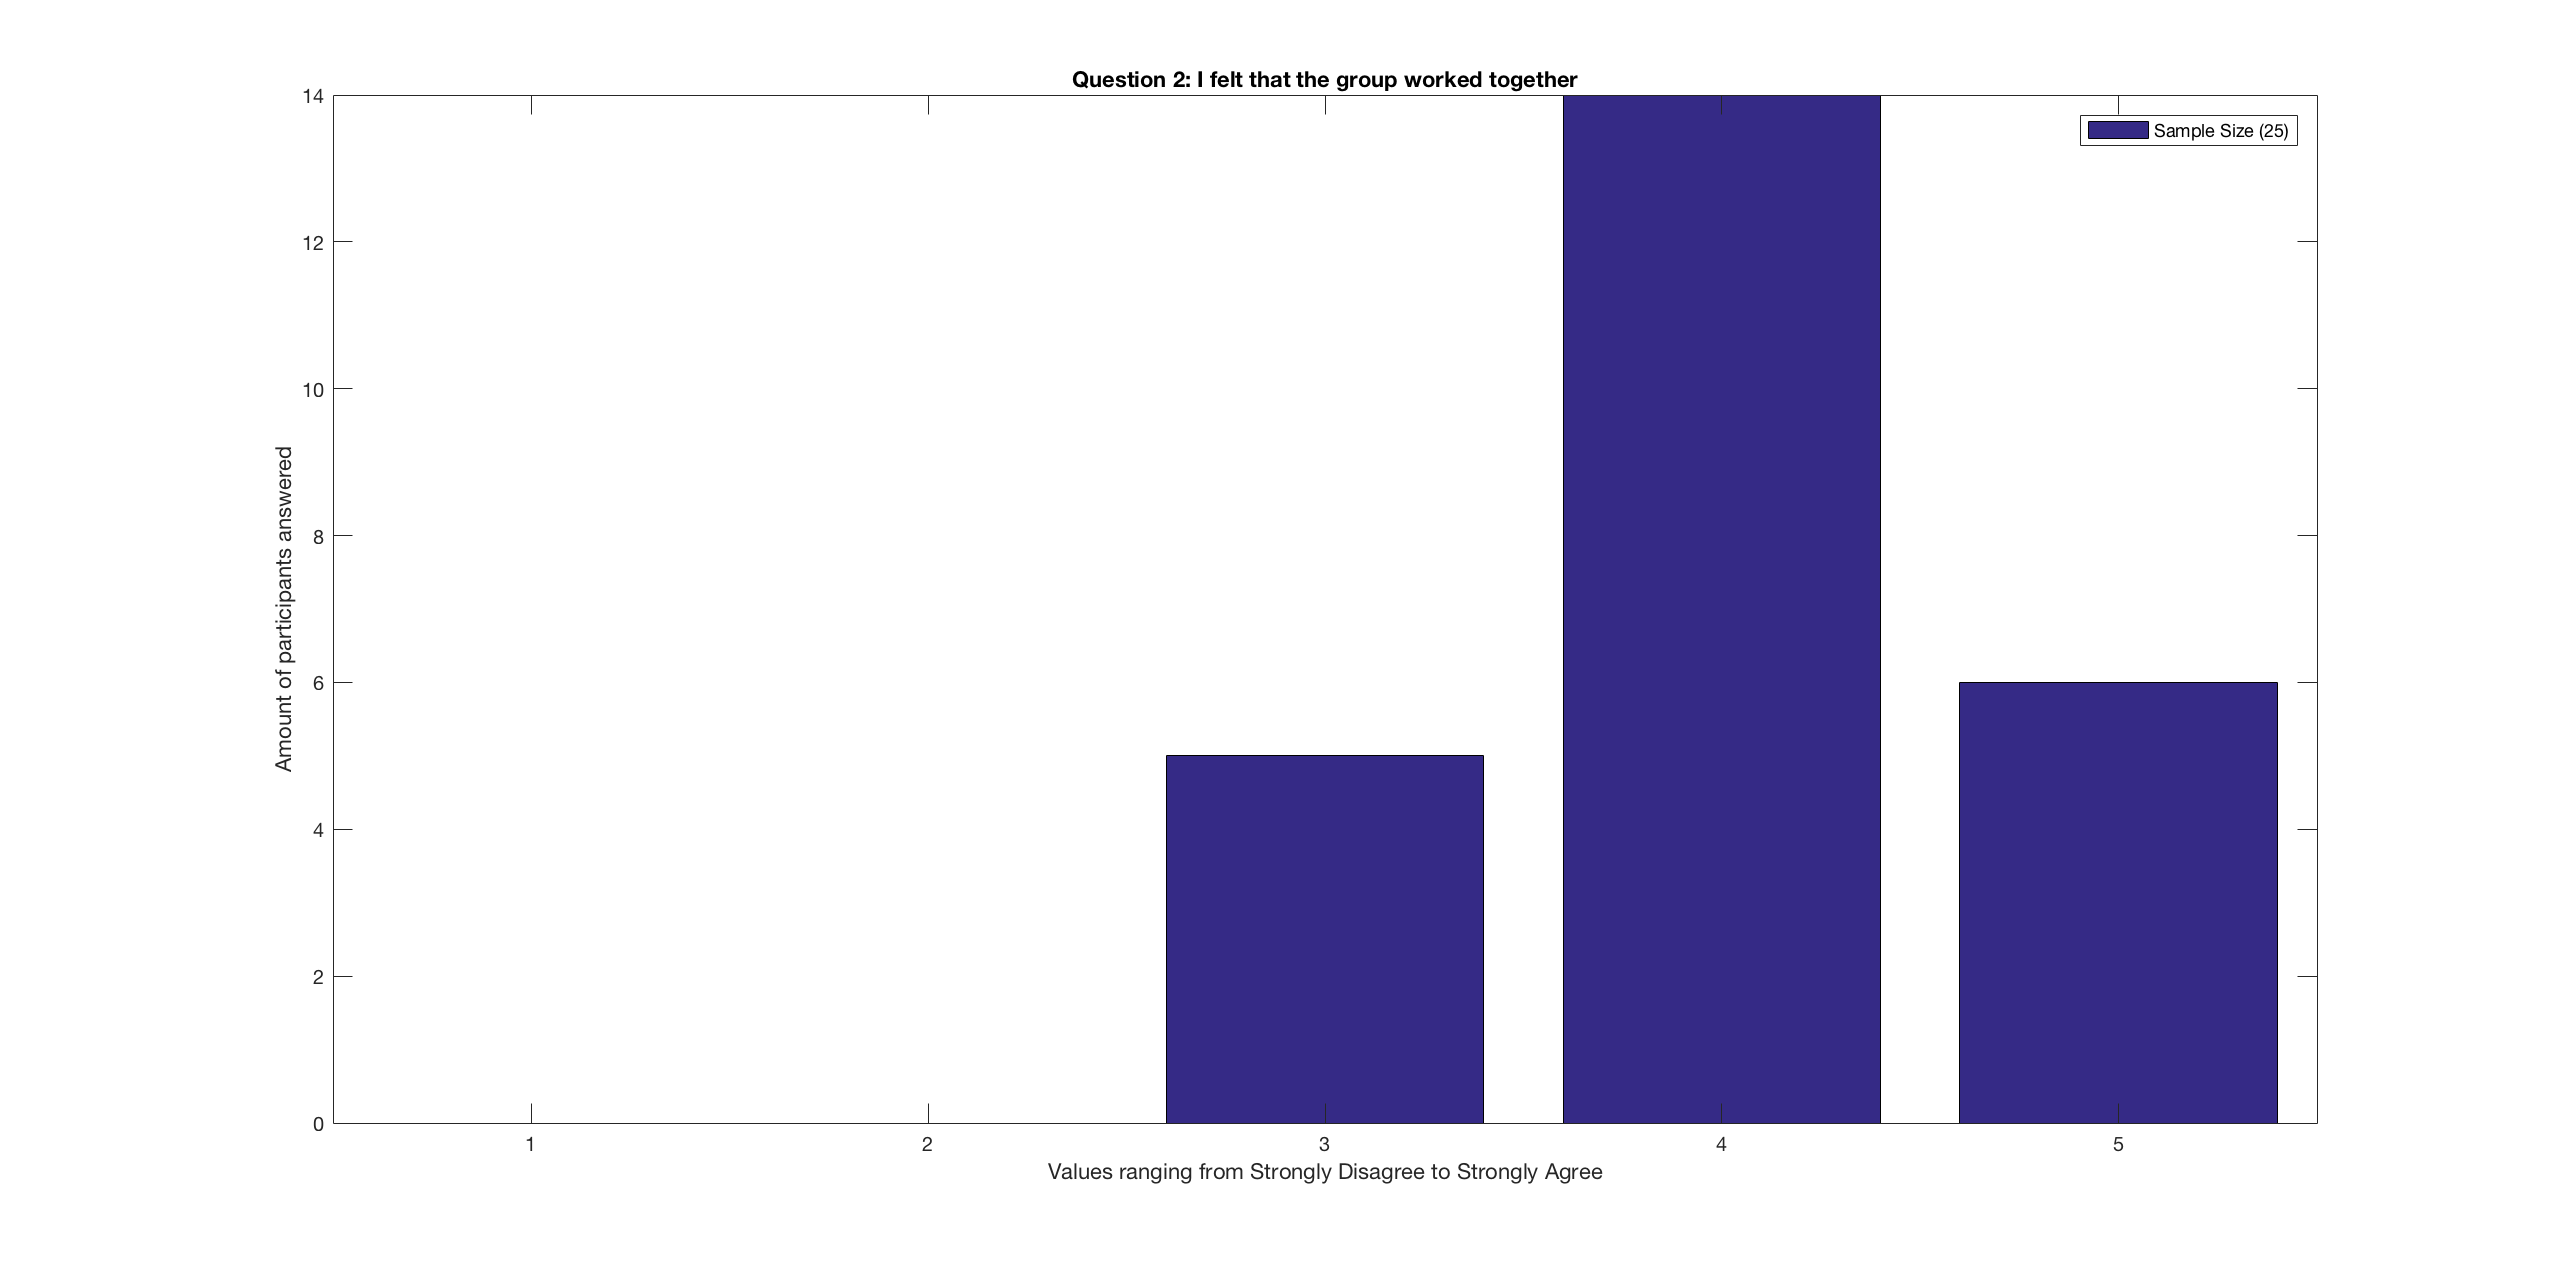
\includegraphics[width=0.9\linewidth]{figure/Appendices/Question2} 
		\caption{Question2}
	\end{figure}

    \begin{figure}[H]
		\centering
		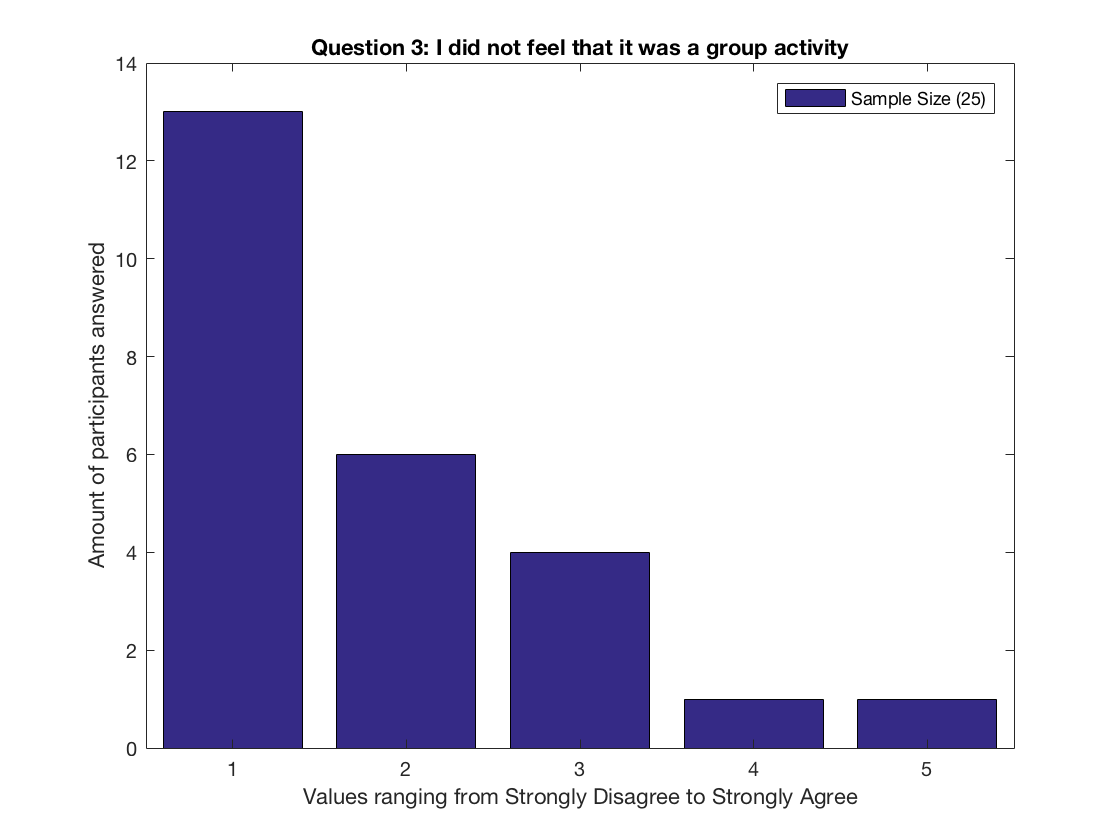
\includegraphics[width=0.9\linewidth]{figure/Appendices/Question3M} 
		\caption{Question3}
	\end{figure}

    \begin{figure}[H]
		\centering
		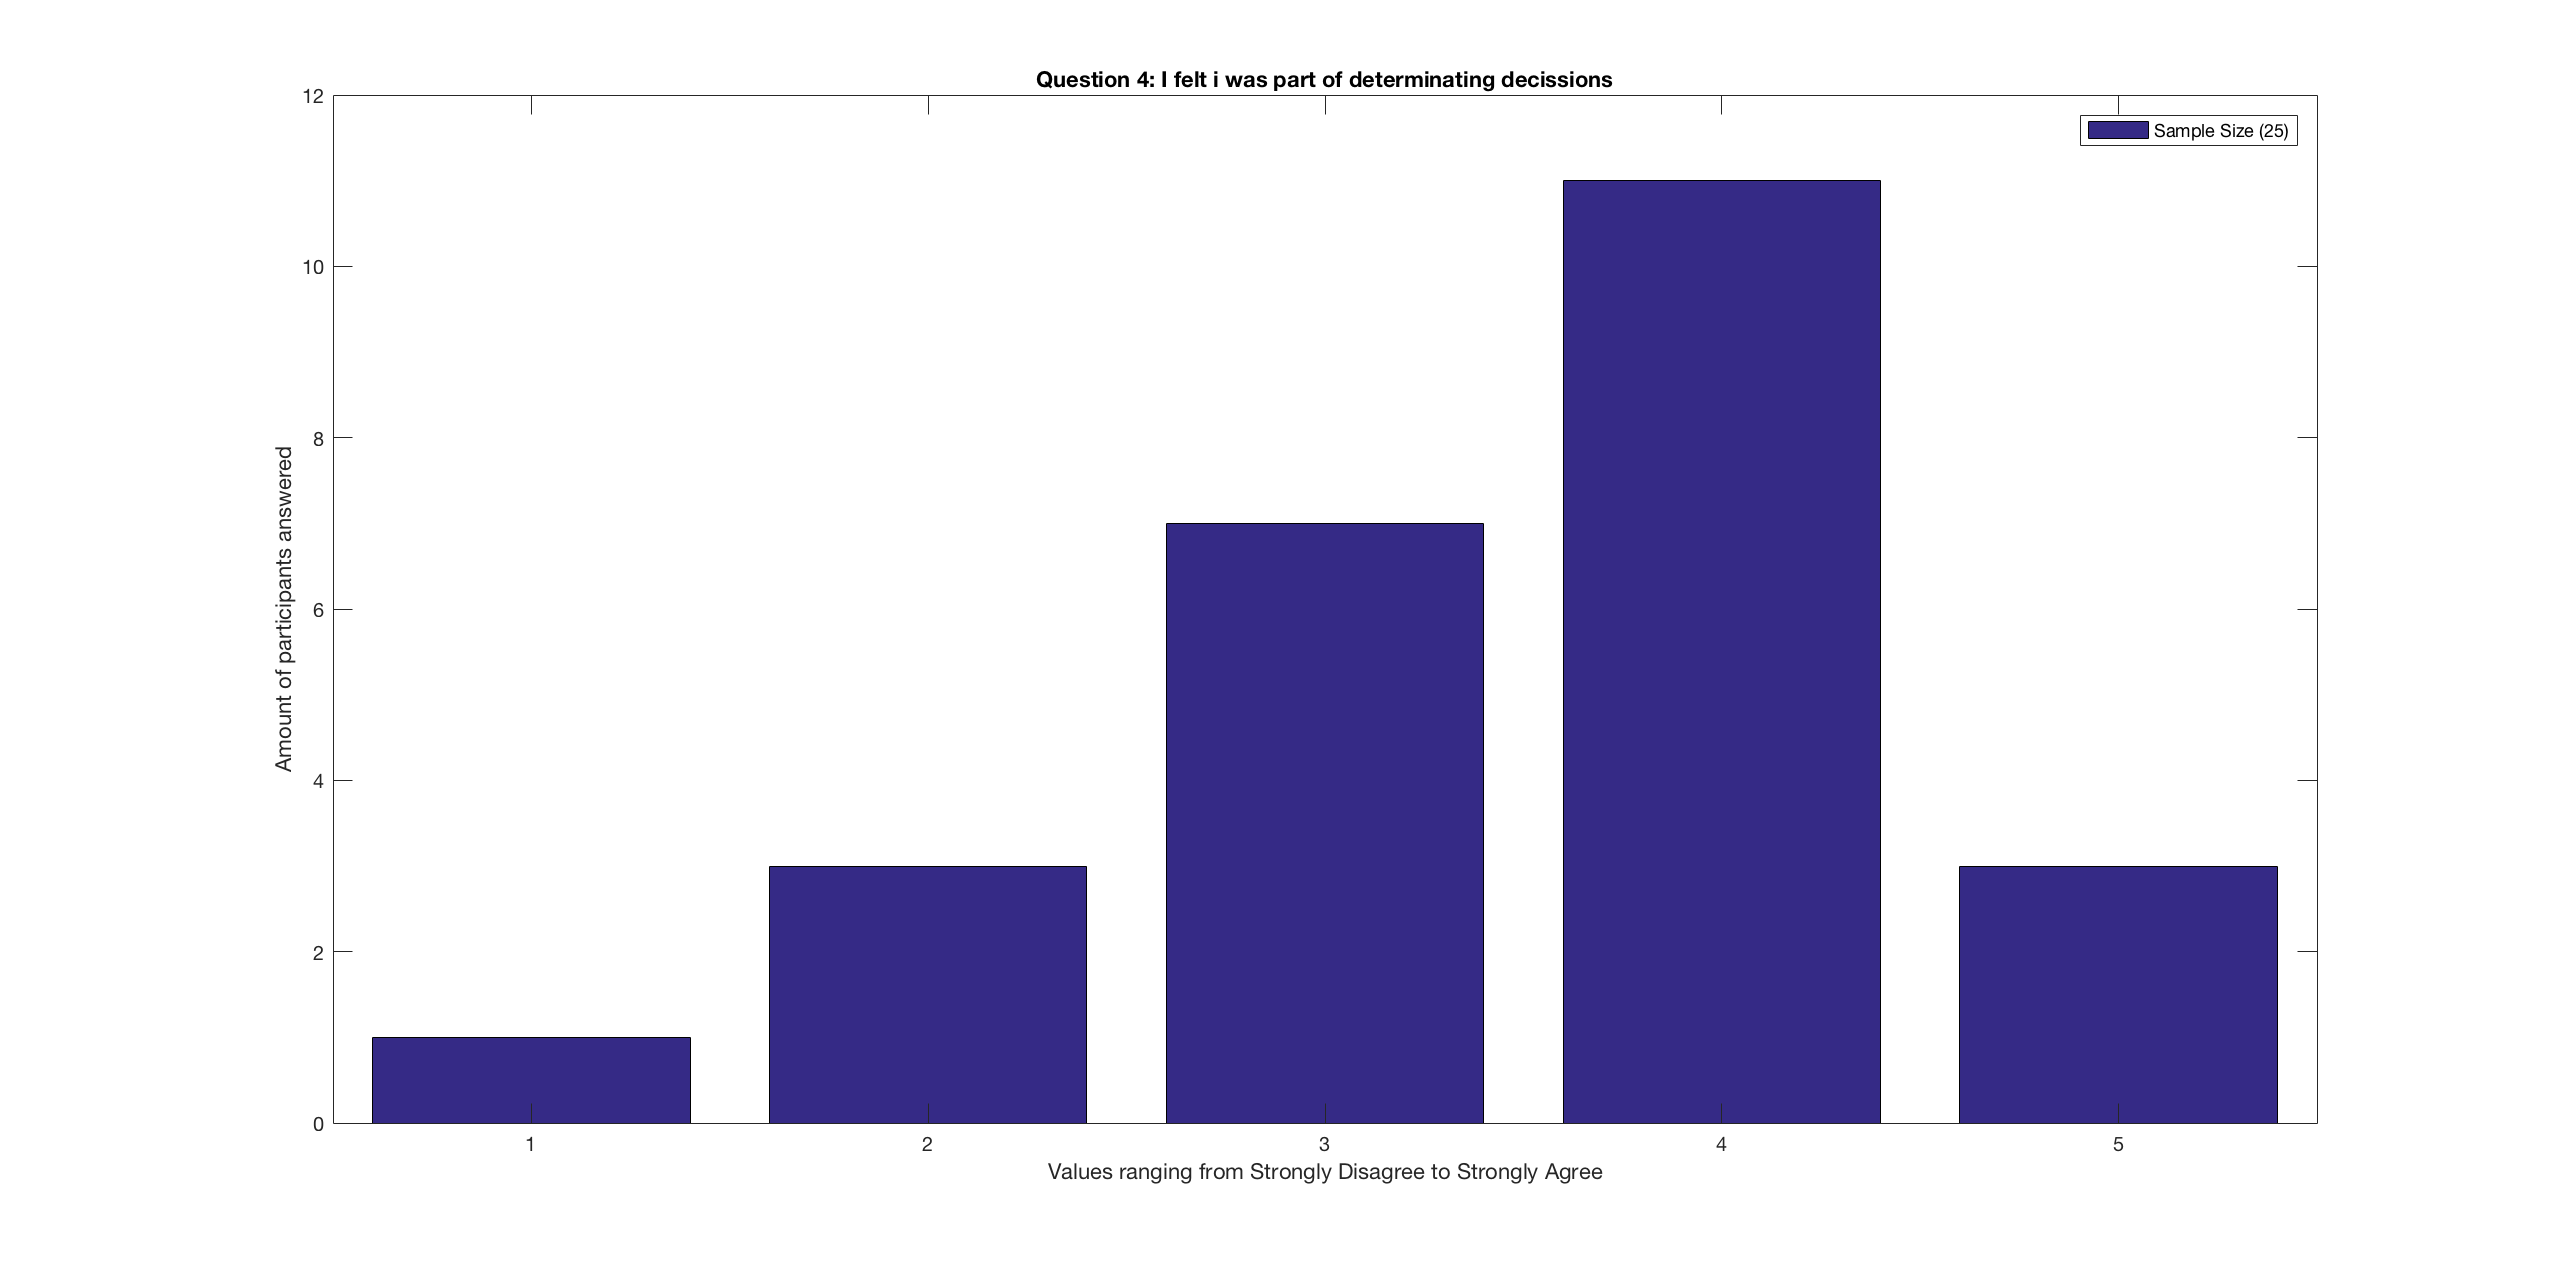
\includegraphics[width=0.9\linewidth]{figure/Appendices/Question4} 
		\caption{Question4}
	\end{figure}

    \begin{figure}[H]
		\centering
		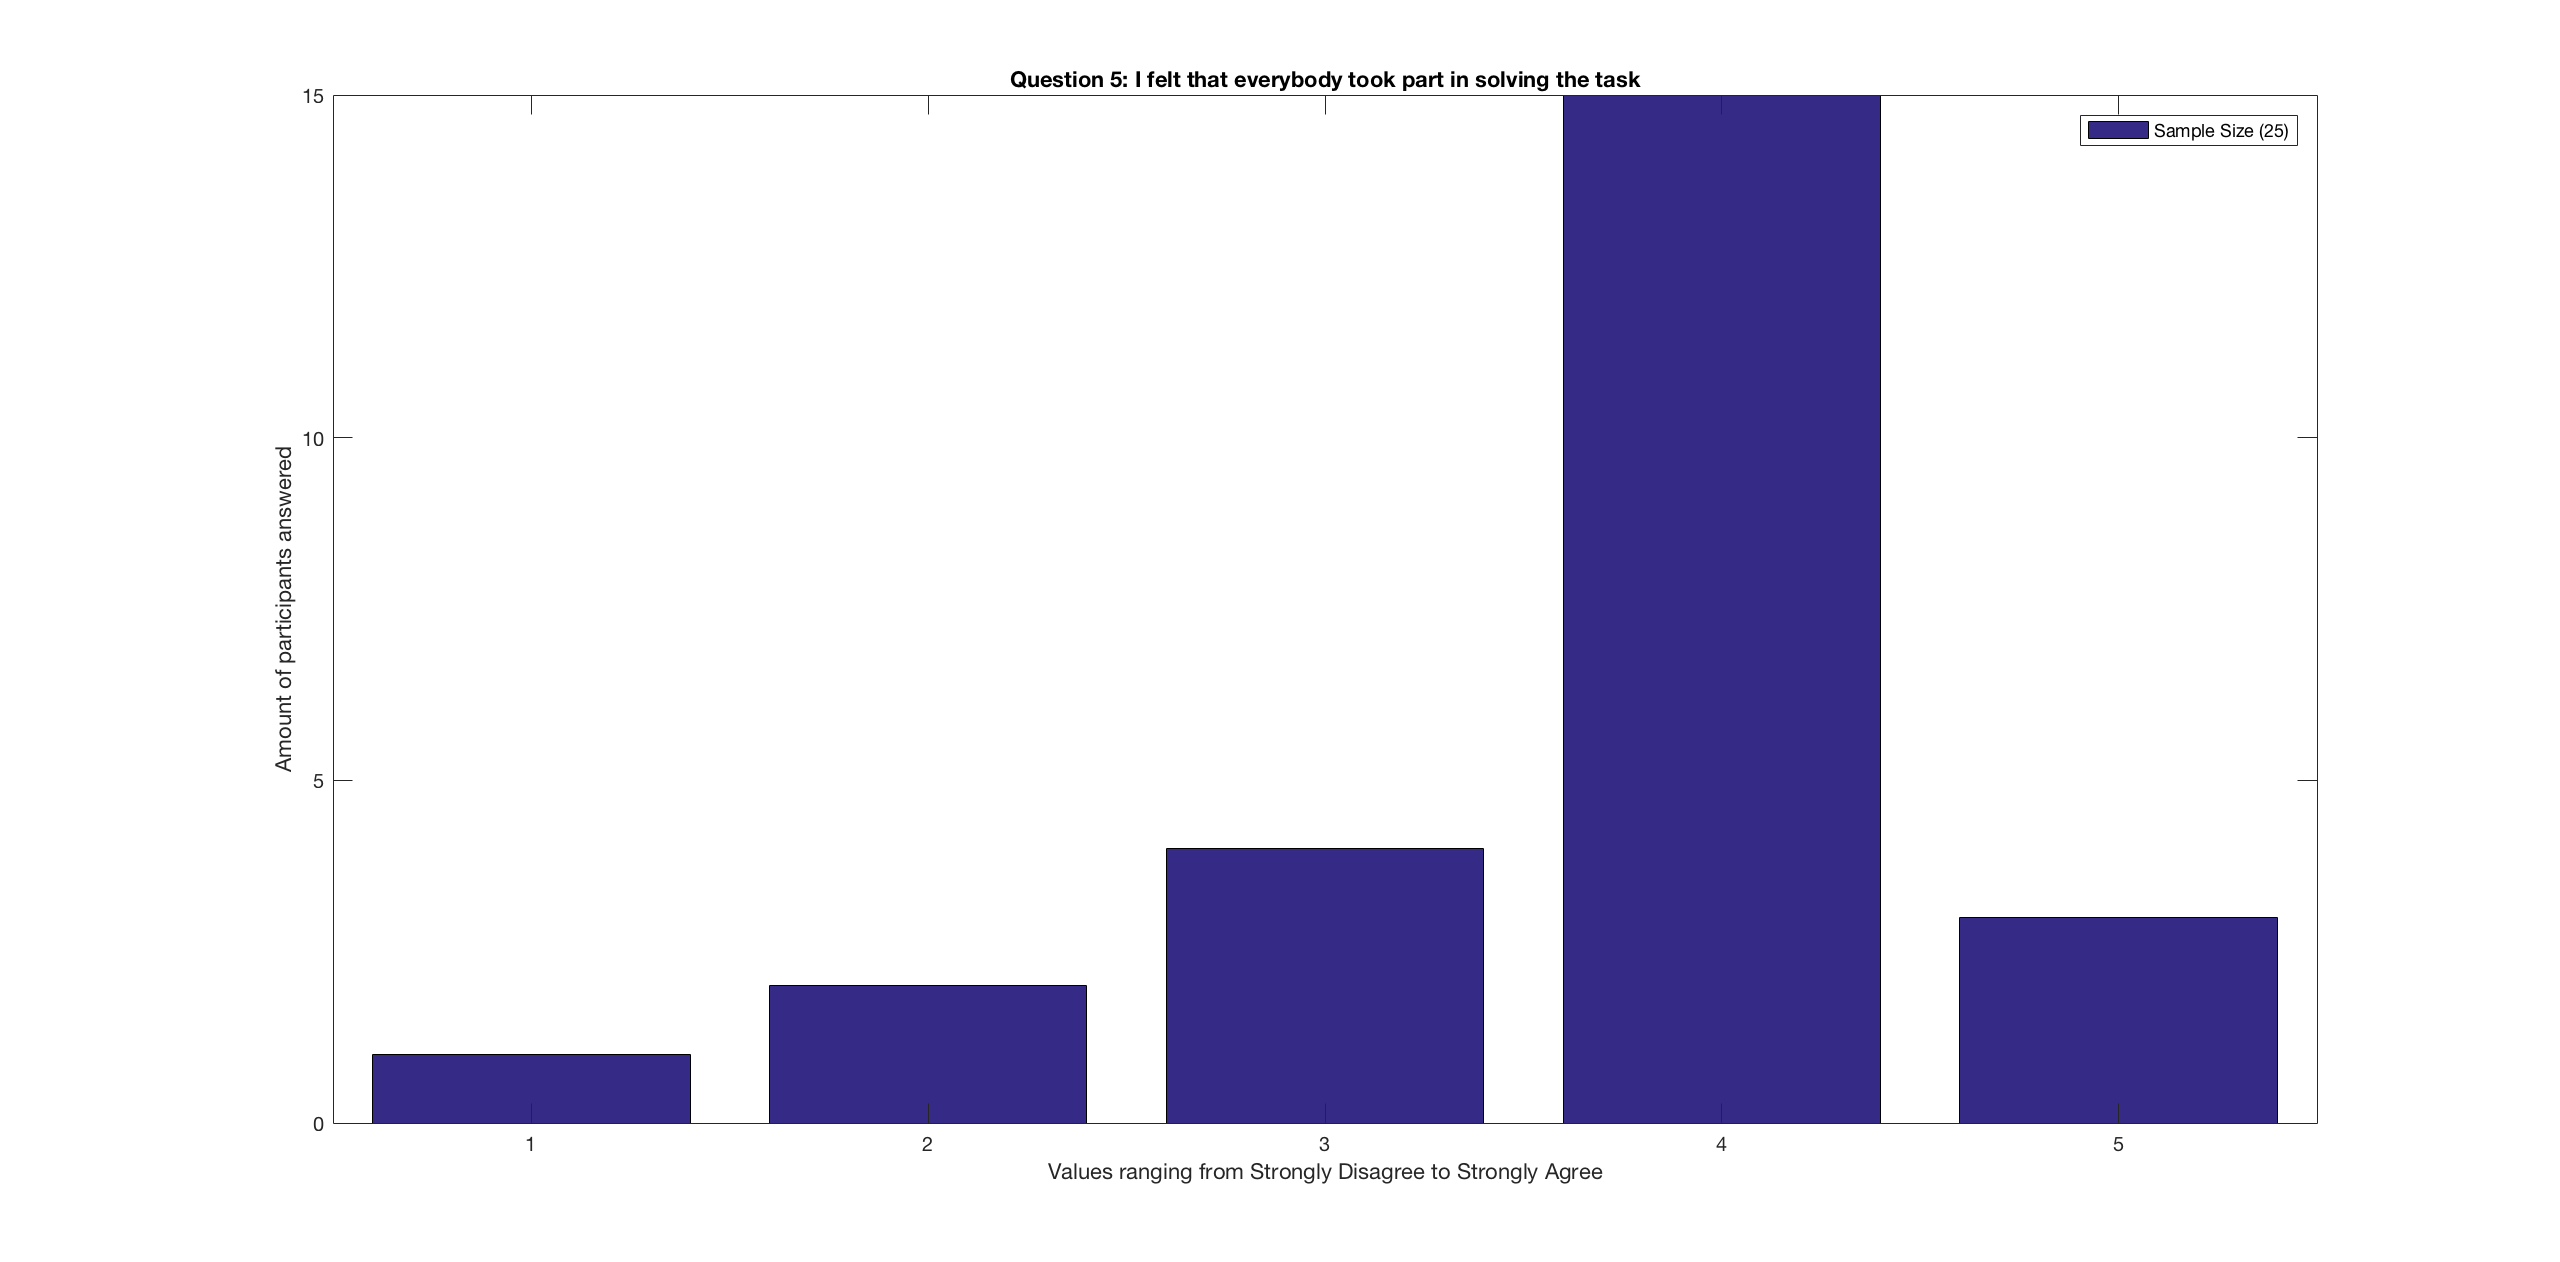
\includegraphics[width=0.9\linewidth]{figure/Appendices/Question5} 
		\caption{Question5}
	\end{figure}

    \begin{figure}[H]
		\centering
		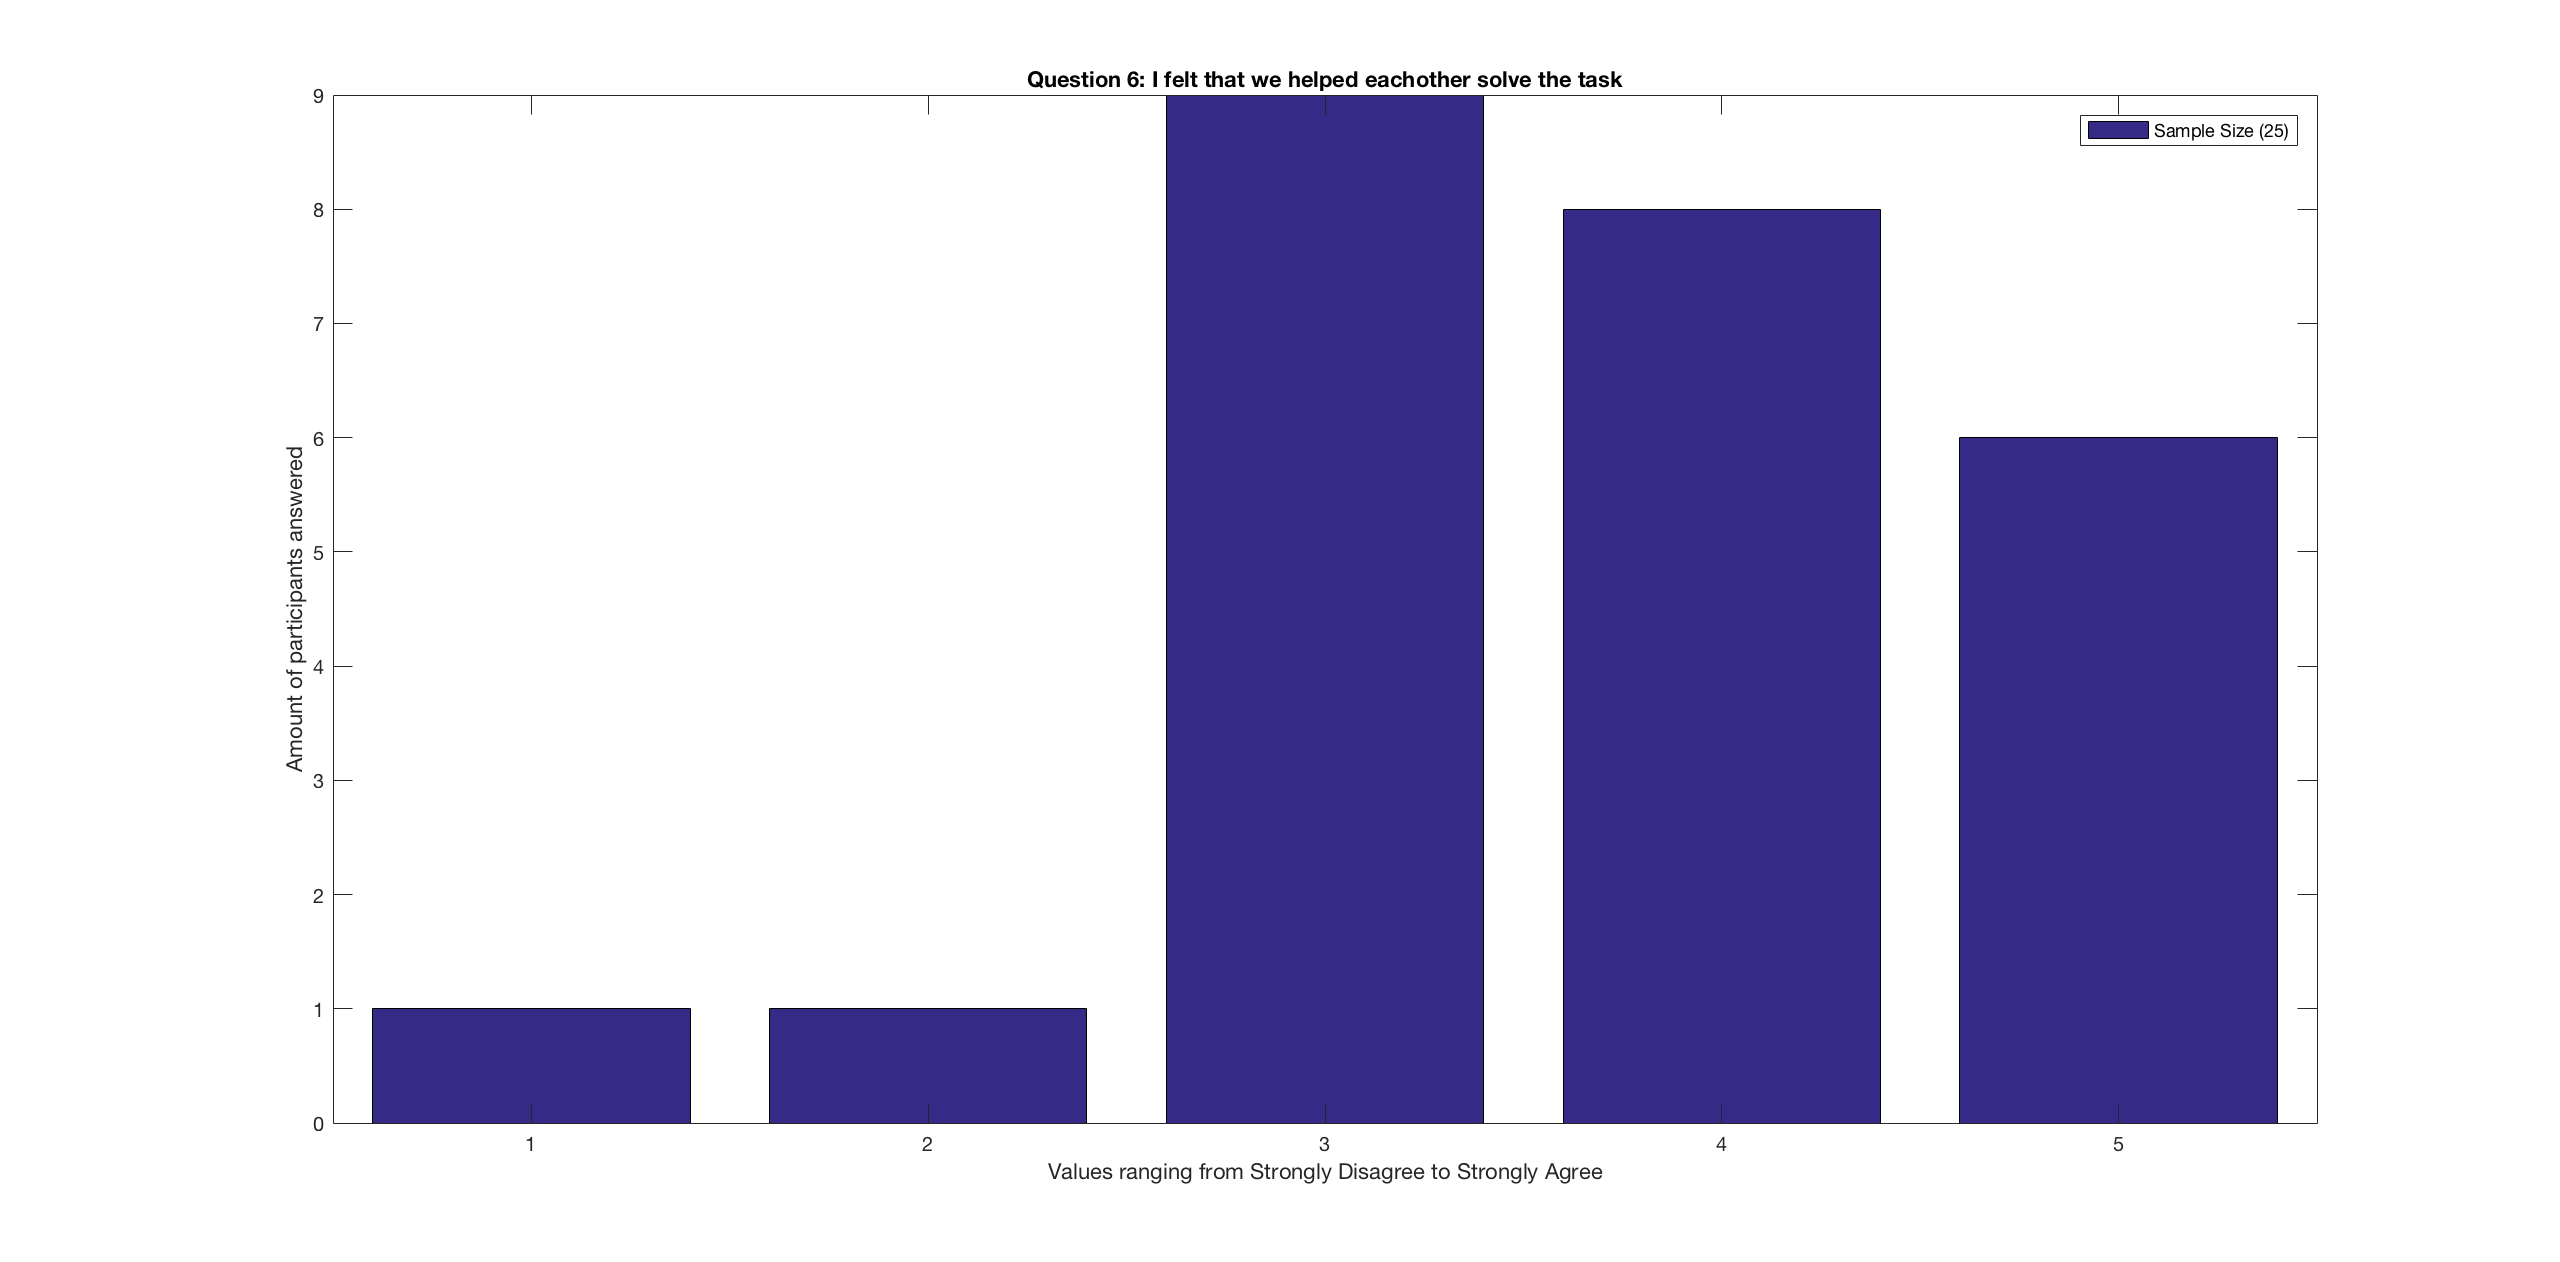
\includegraphics[width=0.9\linewidth]{figure/Appendices/Question6} 
		\caption{Question6}
	\end{figure}

    \begin{figure}[H]
		\centering
		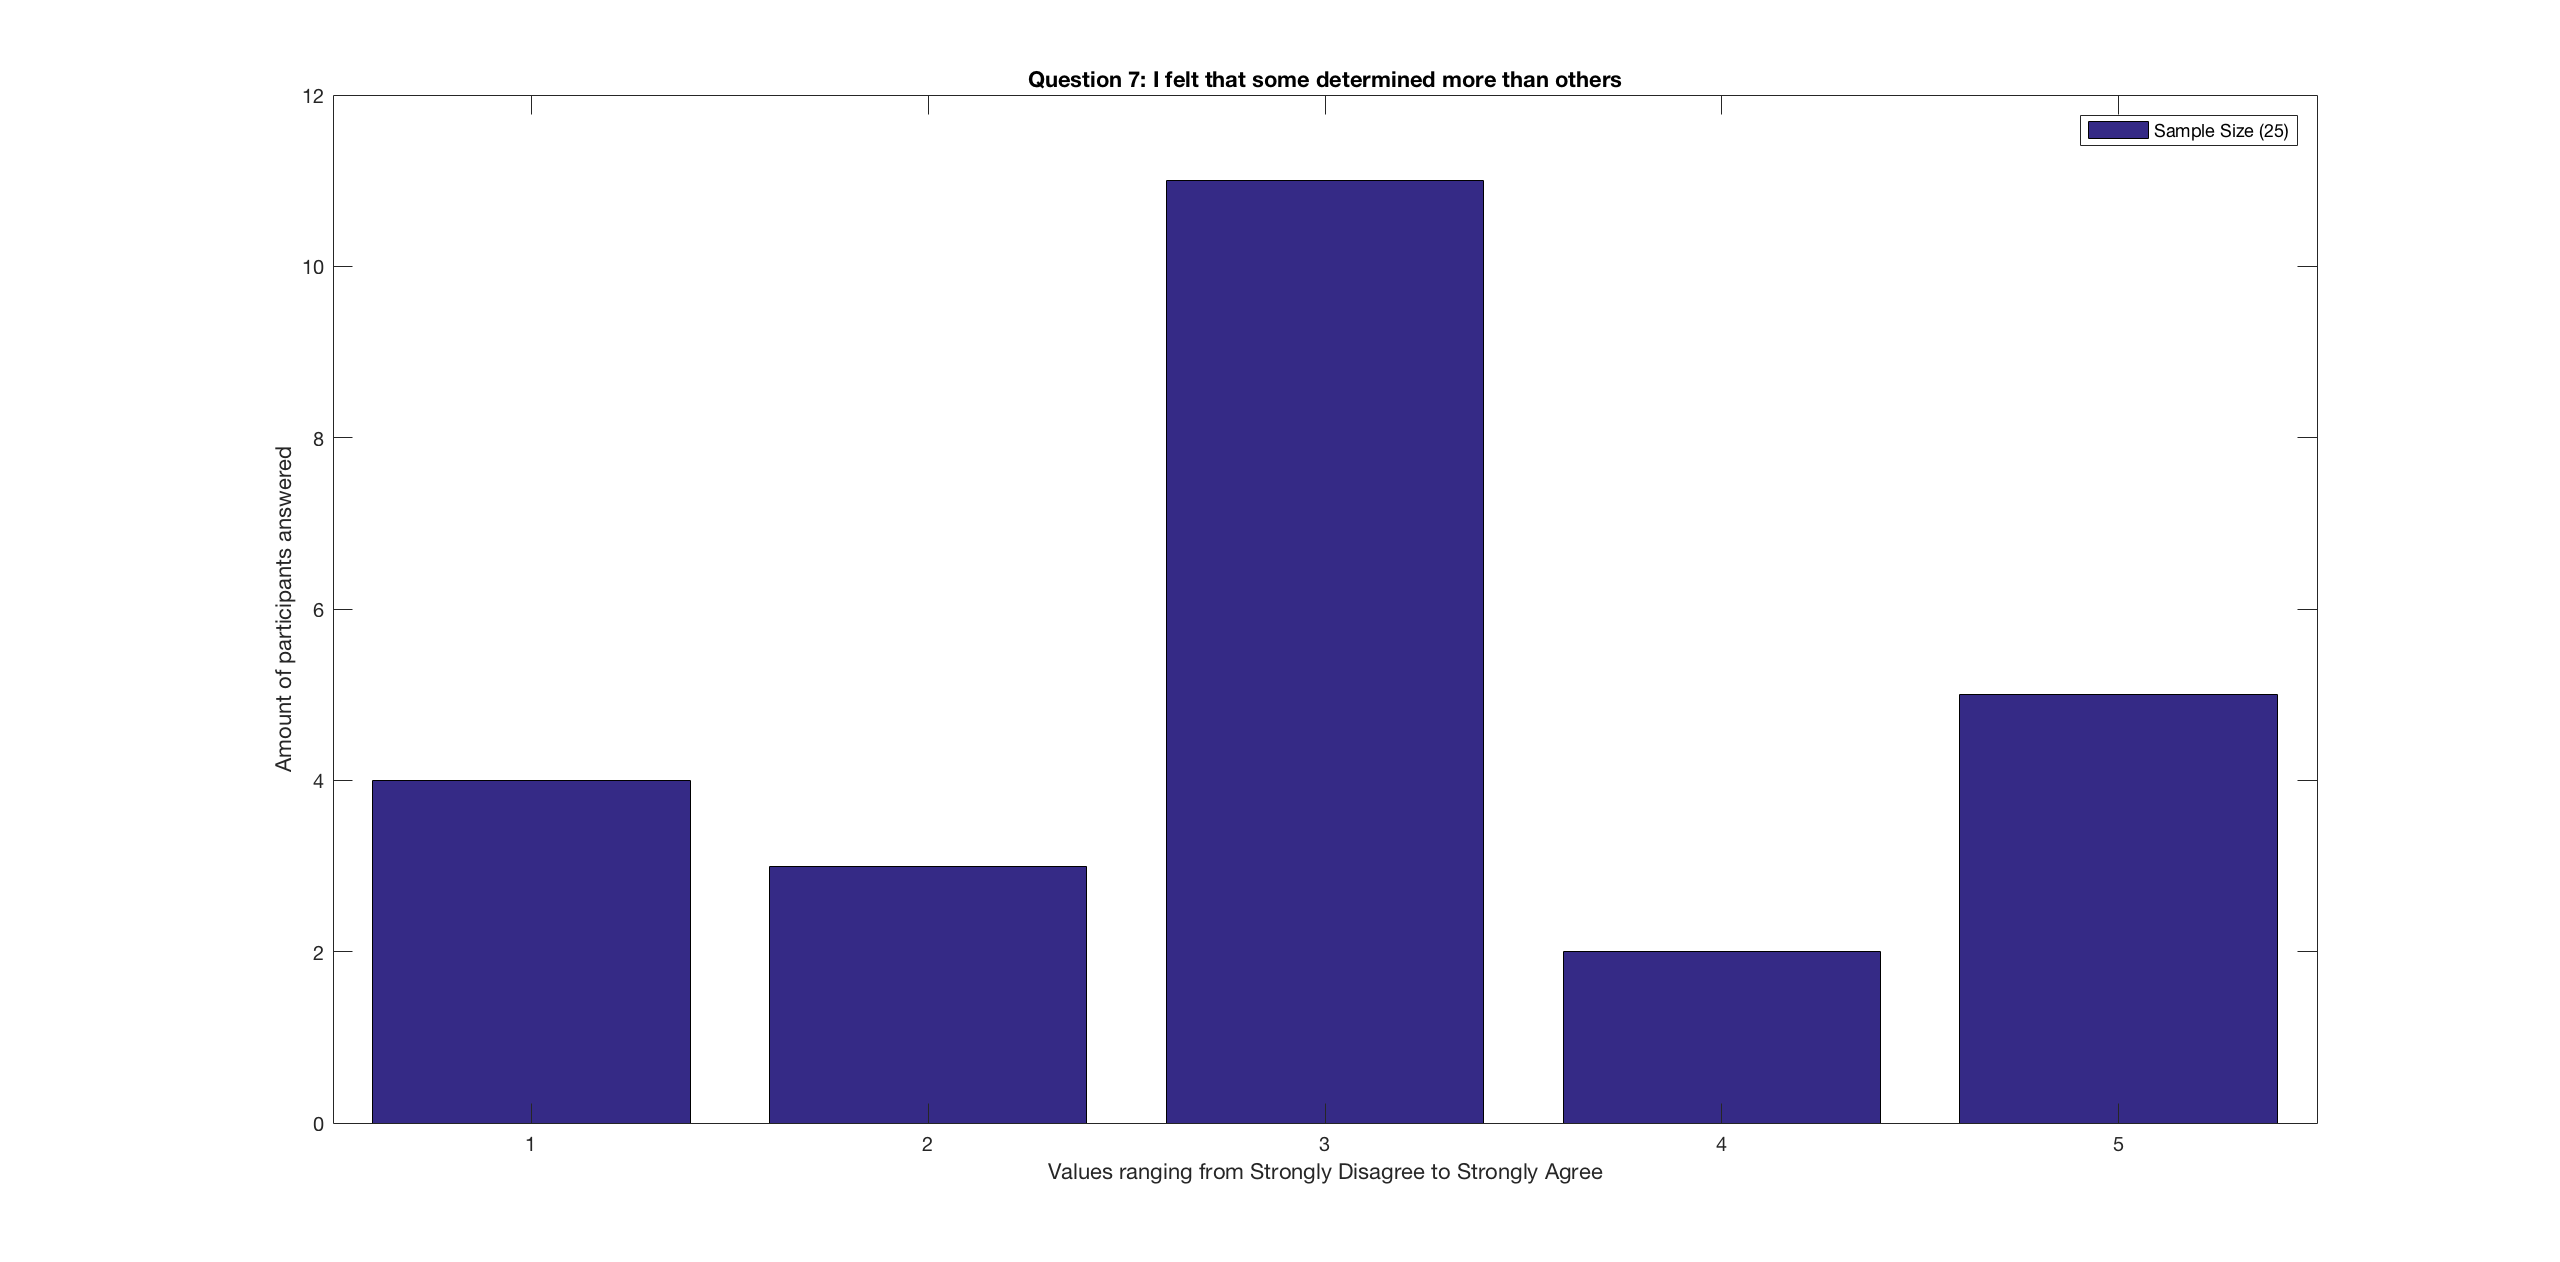
\includegraphics[width=0.9\linewidth]{figure/Appendices/Question7} 
		\caption{Question7}
	\end{figure}

    \begin{figure}[H]
		\centering
		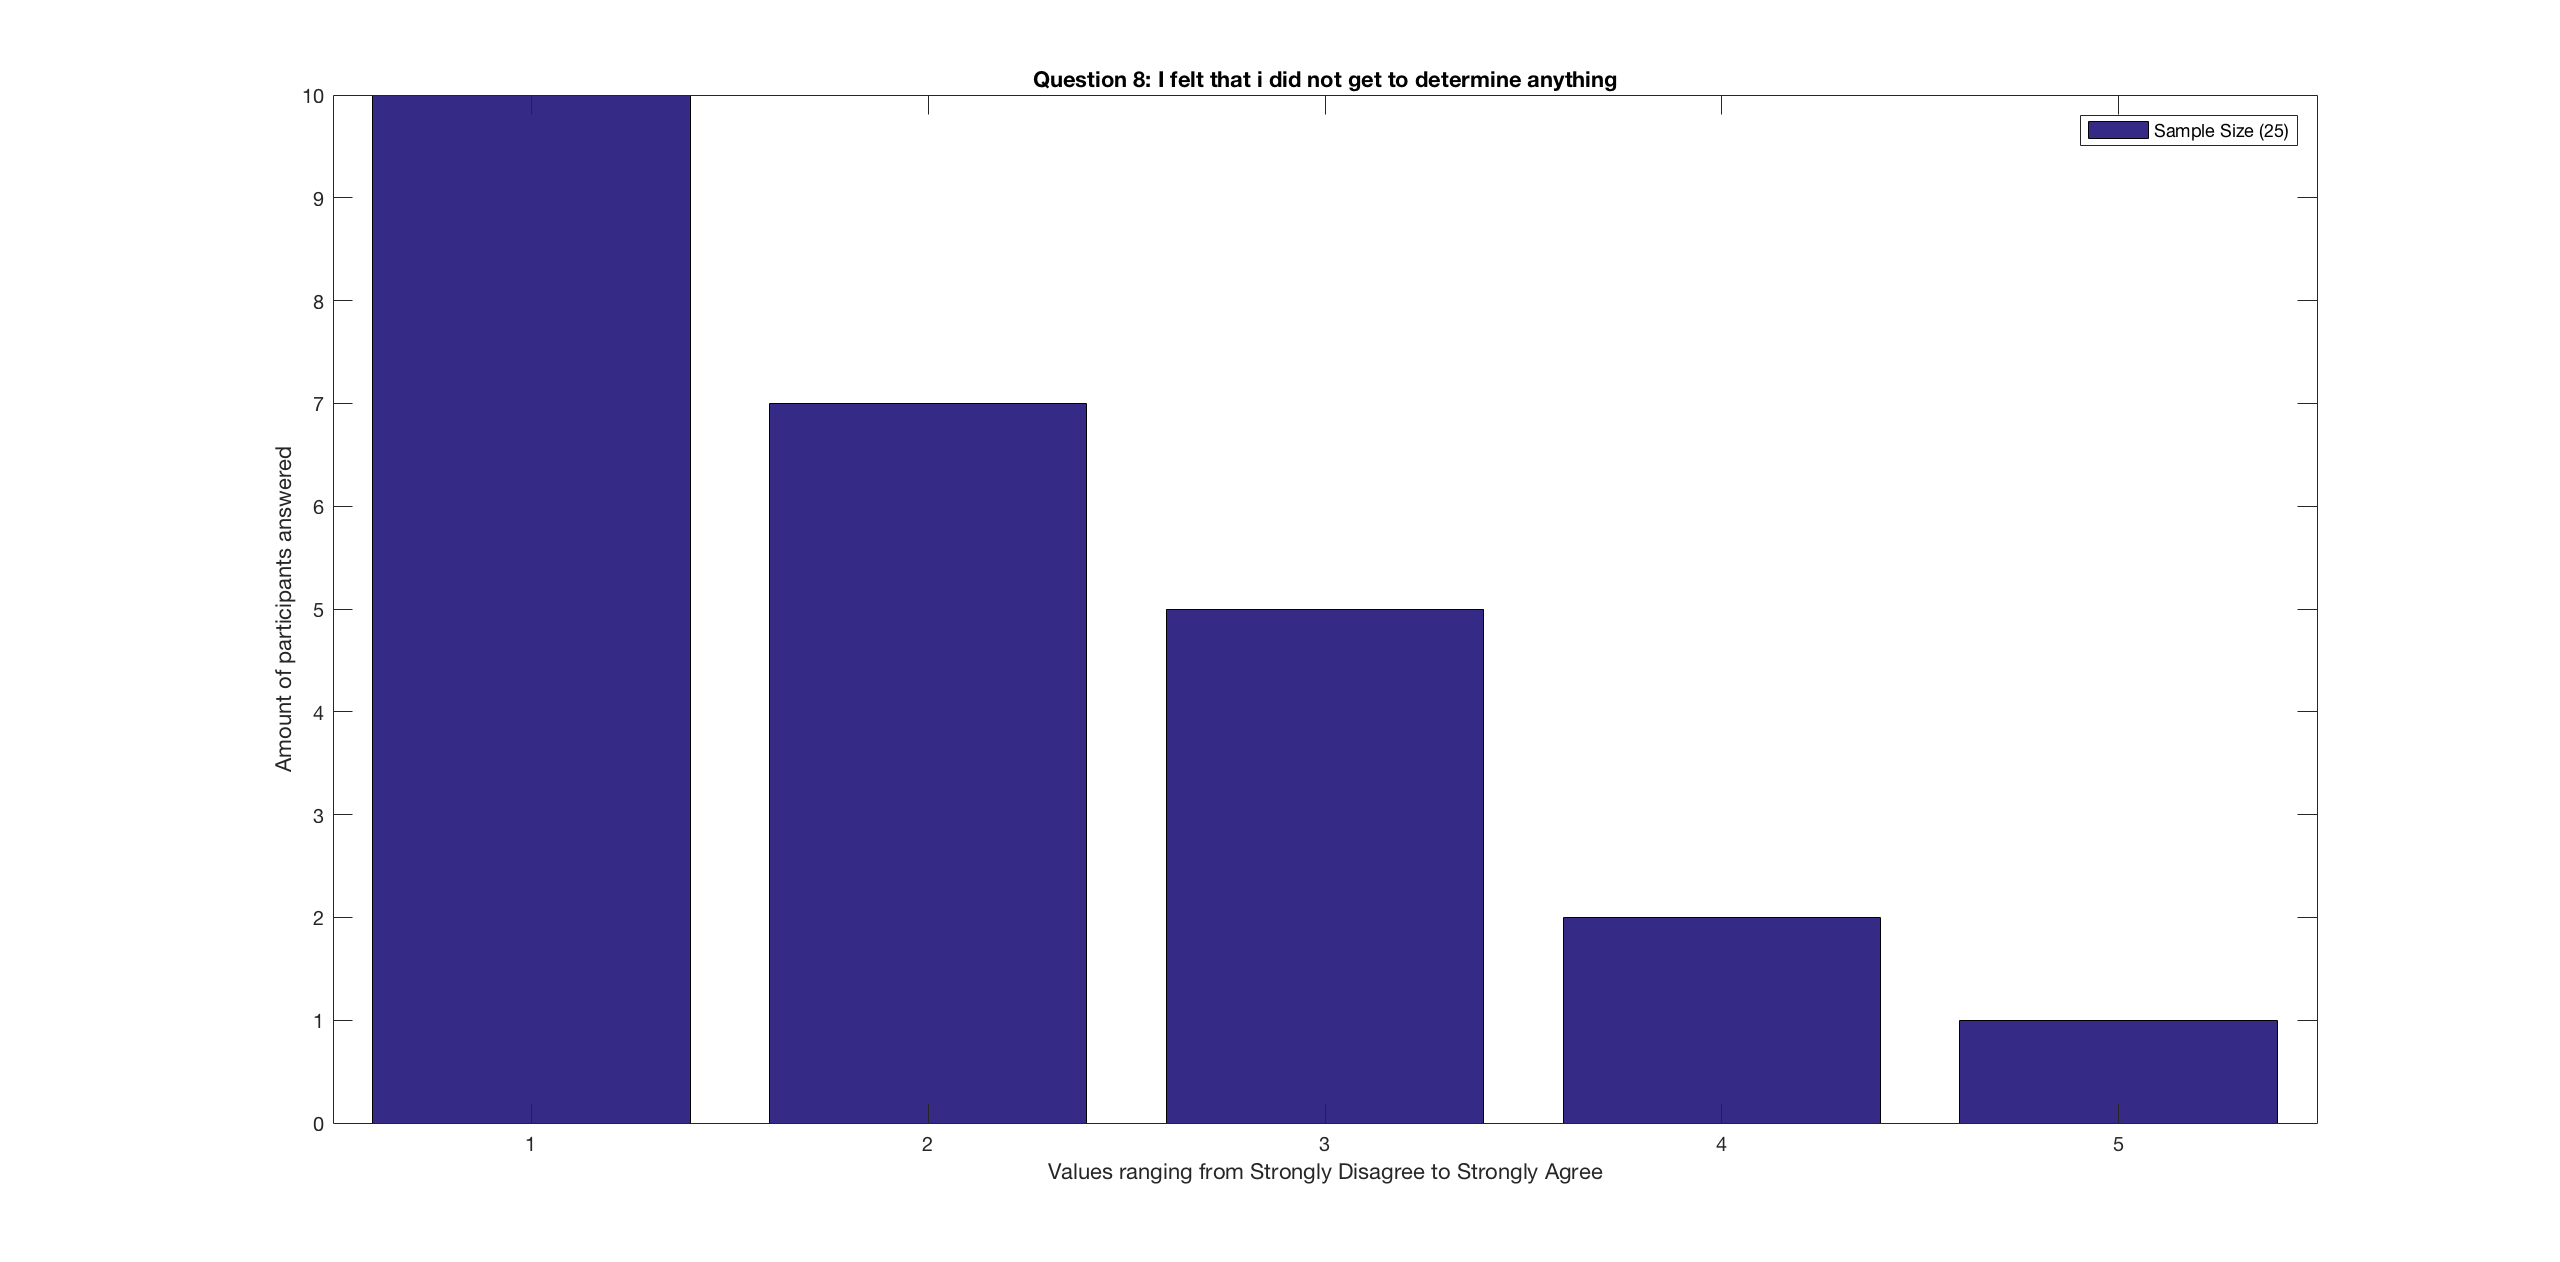
\includegraphics[width=0.9\linewidth]{figure/Appendices/Question8} 
		\caption{Question8}
	\end{figure}

\section{Sus results}\label{appendix:susResults}
\begin{table}[]
	\centering
	\caption{Full table showing the SUS score for each individual test participants and overall mean score.}
	\label{tab:susScoreTableAppendix}
	\begin{tabular}{|c|c|c|c|c|c|l|l|l|l|l|l|}
		\hline
		Participant & Q1 & Q2 & Q3 & Q4 & Q5 & Q6 & Q7 & Q8 & Q9 & Q10 & SUS Score \\ \hline
		1           & 2  & 3  & 2  & 3  & 3  & 2  & 5  & 3  & 1  & 1   & 52.5      \\ \hline
		2           & 1  & 1  & 5  & 1  & 4  & 1  & 5  & 4  & 3  & 1   & 75.0      \\ \hline
		3           & 3  & 4  & 4  & 4  & 5  & 4  & 2  & 5  & 2  & 1   & 45.0      \\ \hline
		4           & 1  & 3  & 3  & 3  & 4  & 2  & 5  & 2  & 4  & 5   & 55.0      \\ \hline
		5           & 1  & 2  & 5  & 1  & 4  & 2  & 4  & 2  & 4  & 1   & 75.0      \\ \hline
		6           & 1  & 4  & 2  & 3  & 4  & 2  & 3  & 4  & 2  & 4   & 37.5      \\ \hline
		7           & 2  & 1  & 5  & 3  & 5  & 4  & 4  & 2  & 4  & 2   & 70.0      \\ \hline
		8           & 2  & 1  & 4  & 1  & 3  & 2  & 5  & 1  & 4  & 1   & 80.0      \\ \hline
		9           & 2  & 2  & 4  & 3  & 4  & 2  & 5  & 2  & 4  & 2   & 70.0      \\ \hline
		10          & 2  & 2  & 4  & 2  & 4  & 1  & 5  & 2  & 5  & 3   & 75.0      \\ \hline
		Total       &    &    &    &    &    &    &    &    &    &     & 63.5      \\ \hline
	\end{tabular}
\end{table}